\documentclass[tikz, border=10pt]{standalone}
\usepackage{tikz}
\usetikzlibrary{shapes.multipart, positioning, arrows.meta, calc, shapes.misc}

\begin{document}
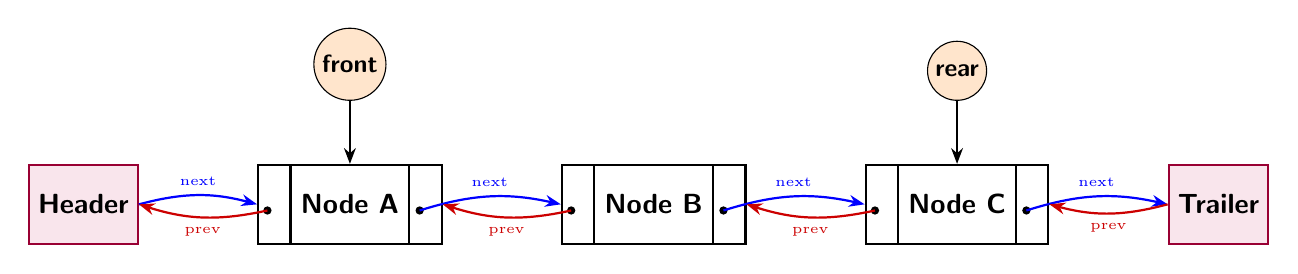
\begin{tikzpicture}[
    dblnode/.style={
        rectangle split,
        rectangle split parts=3,
        rectangle split horizontal,
        draw,
        thick,
        fill=white,
        minimum height=1cm,
        rectangle split part fill={white, white, white},
        font=\sffamily
    },
    sentinel/.style={
        draw,
        rectangle,
        thick,
        fill=purple!10,
        minimum size=1cm,
        font=\sffamily\bfseries,
        draw=purple!80!black
    },
    ptr/.style={
        >={Stealth[length=2mm]},
        ->,
        thick,
        blue
    },
    revptr/.style={
        >={Stealth[length=2mm]},
        ->,
        thick,
        red!80!black
    },
    labelptr/.style={
        >={Stealth[length=2mm]},
        ->,
        thick,
        black
    },
    labelnode/.style={
        draw,
        circle,
        fill=orange!20,
        inner sep=2pt,
        font=\sffamily\bfseries\small
    }
]

    % Nodes
    \node[sentinel] (header) {Header};
    \node[dblnode, right=1.5cm of header] (nodeA) { \nodepart{one} \phantom{x} \nodepart{two} \textbf{Node A} \nodepart{three} \phantom{x}};
    \node[dblnode, right=1.5cm of nodeA] (nodeB) { \nodepart{one} \phantom{x} \nodepart{two} \textbf{Node B} \nodepart{three} \phantom{x}};
    \node[dblnode, right=1.5cm of nodeB] (nodeC) { \nodepart{one} \phantom{x} \nodepart{two} \textbf{Node C} \nodepart{three} \phantom{x}};
    \node[sentinel, right=1.5cm of nodeC] (trailer) {Trailer};

    % Dots in pointer fields
    \fill[black] (nodeA.one) circle (1.5pt);
    \fill[black] (nodeA.three) circle (1.5pt);
    \fill[black] (nodeB.one) circle (1.5pt);
    \fill[black] (nodeB.three) circle (1.5pt);
    \fill[black] (nodeC.one) circle (1.5pt);
    \fill[black] (nodeC.three) circle (1.5pt);

    % Forward Pointers (Next)
    \draw[ptr] (header.east) to[bend left=15] node[midway, above, font=\tiny, text=blue] {next} (nodeA.west);
    \draw[ptr] (nodeA.three) to[bend left=15] node[midway, above, font=\tiny, text=blue] {next} (nodeB.west);
    \draw[ptr] (nodeB.three) to[bend left=15] node[midway, above, font=\tiny, text=blue] {next} (nodeC.west);
    \draw[ptr] (nodeC.three) to[bend left=15] node[midway, above, font=\tiny, text=blue] {next} (trailer.west);

    % Backward Pointers (Prev)
    \draw[revptr] (trailer.west) to[bend left=15] node[midway, below, font=\tiny, text=red!80!black] {prev} (nodeC.east); % Use east for consistency with previous diagrams or logic?
    % Let's use nodeC.east for "prev" target to differentiate from "next" source?
    % Actually previous diagram used node.east for prev target.
    
    \draw[revptr] (nodeC.one) to[bend left=15] node[midway, below, font=\tiny, text=red!80!black] {prev} (nodeB.east);
    \draw[revptr] (nodeB.one) to[bend left=15] node[midway, below, font=\tiny, text=red!80!black] {prev} (nodeA.east);
    \draw[revptr] (nodeA.one) to[bend left=15] node[midway, below, font=\tiny, text=red!80!black] {prev} (header.east);

    % Front and Rear Pointers
    % Front points to Node A (first element)
    \node[labelnode, above=0.8cm of nodeA] (front) {front};
    \draw[labelptr] (front) -- (nodeA.north);

    % Rear points to Node C (last element)
    \node[labelnode, above=0.8cm of nodeC] (rear) {rear};
    \draw[labelptr] (rear) -- (nodeC.north);

\end{tikzpicture}
\end{document}
